% !TeX root = ../main.tex
% Add the above to each chapter to make compiling the PDF easier in some editors.

\chapter{Methodology}\label{chapter:methodology}

This chapter covers which problem the thesis tackles, how the data used within the different experiments is generated, what the actual data looks like,
which solver-preconditioner classes are used, which features are selected and why, and describes the architecture used in the PyTorch model.

\section{Problem Formulation}\label{sec:problem-formulation}

The goal of the thesis is to evaluate the usability of CNNs for a pipeline that tries to predict the solver-preconditioner
pair that minimises solve time subject to convergence in a large sparse equation in the form of $Ax = b$, where
$A \in \mathbb{R}^{n \times n}$, $b \in \mathbb{R}^{n \times 1}$, and $x \in \mathbb{R}^{n \times 1}$.
To determine the usability an architecture similar to that in the MM-AutoSolver~\cite{xiong2025mmautosolver} paper is introduced initially, which is
then modified in certain aspects like the chosen features and the approach of the CNN implementation.
These changes are done with the goal in mind to achieve the best possible prediction outcome while also improving the overall failure rates and average speedups
of the resulting models which allows them to be used in a complete pipeline.

\section{Dataset Construction}\label{sec:dataset}

The dataset is constructed by combining SuiteSparse~\cite{davis2011university} matrices with synthetically generated matrices and saving the information needed for
further processing into an HDF5 file.
For the dataset a cap on winning solver-preconditioner pairs is introduced to counter a certain bias towards overrepresented pairs in the training phase.
For the dataset used in the experiments this cap was 600, while the minimum of wins for a pair was 250.

\subsection{Synthetic Data Generation}\label{subsec:synthetic-datagen}

The synthetic data generation evolved while testing and generating datasets, in the end 37 different generator buckets
were defined in the process.
These focus on generating matrices with structural properties for which specific solver-preconditioner pairs are theoretically expected to perform well;
the actual winner is always determined empirically by benchmarking.
Table~\ref{tab:generator-buckets} lists all generator functions grouped by structural property.
In practice, however, this worked only partially, as even though some solver wins increased, in most cases the intended target solvers were still
outperformed by certain more dominant solver-preconditioner pairs.
A more systematic bucket design falls outside the scope of this thesis and these downsides are therefore accepted as limitations.
For generators where only the size changes which solver-preconditioner pair has the highest chance of winning, different buckets
that generate specific sizes with a certain generator function are introduced.
If these generators produce large matrices, they have a lower chance to be used as they
dramatically increase the runtime of the data generation.
In the current state, the generators generate matrices with $n$ ranging from 100 to 125{,}000.

\begin{table}[H]
  \centering
  \caption{Synthetic generator buckets grouped by structural matrix property.
           Size variants of the same generator function are merged into one row.
           Solver requirements follow~\cite{saad2003iterative}: CG requires SPD (Ch.\,6),
           MINRES/SYMMLQ require symmetry (Ch.\,6), GMRES and BiCGS variants apply to
           nonsymmetric systems (Ch.\,7).
           Primary targets are theoretically motivated and empirically confirmed.}
  \label{tab:generator-buckets}
  \small
  \begin{tabular}{@{}llp{4.5cm}@{}}
    \toprule
    \textbf{Generator function} & \textbf{$n$ range} & \textbf{Primary target(s)} \\
    \midrule
    \multicolumn{3}{@{}l@{}}{\textit{Symmetric positive-definite (SPD)}} \\[2pt]
    \texttt{random\_spd}               & 100–1\,000      & \texttt{cg+\{ilu, eisenstat, bjacobi\}} \\
    \texttt{poisson\_2d}               & 100–90\,000     & \texttt{cg+*, minres+gamg, fcg+gamg} \\
    \texttt{poisson\_3d}               & 125–125\,000    & \texttt{cg+*, minres+gamg, fcg+gamg} \\
    \texttt{anisotropic\_poisson\_2d}  & 100–40\,000     & \texttt{cg+ilu, fcg+gamg} \\
    \texttt{anisotropic\_poisson\_3d}  & 1\,700–27\,000  & \texttt{fcg+gamg} \\
    \midrule
    \multicolumn{3}{@{}l@{}}{\textit{Symmetric indefinite}} \\[2pt]
    \texttt{shifted\_spd}              & 100–10\,000     & \texttt{symmlq+*, cr+*} \\
    \texttt{helmholtz\_2d}             & 400–10\,000     & \texttt{symmlq+*, minres+gamg} \\
    \texttt{shifted\_poisson\_2d}      & 400–22\,500     & \texttt{symmlq+sor} \\
    \texttt{sym\_banded\_indefinite}   & 1\,000–12\,000  & \texttt{symmlq+sor} \\
    \texttt{sym\_banded\_mild}         & 800–18\,000     & \texttt{symmlq+sor} \\
    \texttt{sym\_indef\_deep}          & 200–12\,000     & \texttt{symmlq+jacobi} \\
    \midrule
    \multicolumn{3}{@{}l@{}}{\textit{Non-symmetric}} \\[2pt]
    \texttt{random\_nonsymmetric}      & 100–20\,000     & \texttt{fbcgsr+jacobi, bcgsl+none} \\
    \texttt{convection\_diffusion\_2d} & 100–63\,000     & \texttt{fbcgsr+ilu, cgs+gamg, fgmres+gamg} \\
    \texttt{convection\_diffusion\_3d} & 1\,000–43\,000  & \texttt{fbcgsr+ilu, bcgsl+asm, cgs+gamg} \\
    \texttt{random\_banded}            & 500–20\,000     & \texttt{cr+ilu, cg+ilu} \\
    \texttt{barely\_dominant\_nonsym}  & 200–8\,000      & \texttt{dgmres+none} \\
    \bottomrule
  \end{tabular}
\end{table}

Regarding the benchmarking, all solver pairs are run against a matrix after its generation.
A specific timeout is set, after which a solver pair is marked as non-converging, also if the maximum number of iterations is exceeded
the pair is marked as non-converging.
Some solvers do not work, or only work, on symmetric matrices; they are therefore not run on these specific ones.
A pair is valid and gets saved with its solve time if the result is within a certain tolerance.
The label a matrix gets in the end is only the fastest solver-preconditioner pair, the so-called winner.

For each matrix, the matrix itself, the features, and all the pairs with solve time or an entry for non-convergence are stored.

\subsection{SuiteSparse Benchmark Matrices}\label{subsec:SuiteSparse}

The SuiteSparse dataset generation differs only in the storage of the matrices.
Since they are downloaded and stored as \texttt{.mtx} files, the storage of the full matrices in the HDF5 dataset file does not make sense
and is therefore omitted to save space.
A separate folder for the \texttt{.mtx} files is used as a cache, which reduces storage requirements while keeping the dataset portable.

\subsection{Dataset Statistics}\label{subsec:dataset-stats}

The dataset contains 9711 matrices in total, split into 8742 training and 969 validation
samples (90/10 stratified split, seed 42).
Of these, 559 (5.8\%) originate from SuiteSparse; the remainder are synthetically generated.

Table~\ref{tab:class-distribution} shows the per-class sample counts: 13 of the 19
solver-preconditioner pairs reached the cap of 600 samples each, while the remaining six
are rarer winners in the benchmarking and therefore underrepresented.

\begin{table}[H]
  \centering
  \caption{Class distribution in the full dataset (9711 samples).
           The label of each matrix is the fastest converging solver-preconditioner pair.
           Classes are capped at 600.}
  \label{tab:class-distribution}
  \begin{tabular}{clrr}
    \toprule
    Rank & Solver + Preconditioner & Count & \% \\
    \midrule
     1 & \texttt{cr+ilu}           & 600 & 6.2 \\
     2 & \texttt{cg+eisenstat}     & 600 & 6.2 \\
     3 & \texttt{cg+bjacobi}       & 600 & 6.2 \\
     4 & \texttt{fbcgsr+jacobi}    & 600 & 6.2 \\
     5 & \texttt{gmres+gamg}       & 600 & 6.2 \\
     6 & \texttt{fgmres+gamg}      & 600 & 6.2 \\
     7 & \texttt{cg+ilu}           & 600 & 6.2 \\
     8 & \texttt{cr+jacobi}        & 600 & 6.2 \\
     9 & \texttt{minres+gamg}      & 600 & 6.2 \\
    10 & \texttt{fbcgsr+ilu}       & 600 & 6.2 \\
    11 & \texttt{cr+eisenstat}     & 600 & 6.2 \\
    12 & \texttt{bcgsl+none}       & 600 & 6.2 \\
    13 & \texttt{symmlq+icc}       & 600 & 6.2 \\
    14 & \texttt{bcgsl+asm}        & 428 & 4.4 \\
    15 & \texttt{dgmres+none}      & 354 & 3.6 \\
    16 & \texttt{cgs+gamg}         & 336 & 3.5 \\
    17 & \texttt{fcg+gamg}         & 290 & 3.0 \\
    18 & \texttt{symmlq+jacobi}    & 253 & 2.6 \\
    19 & \texttt{symmlq+sor}       & 250 & 2.6 \\
    \midrule
    & Total                        & 9711 & 100.0 \\
    \bottomrule
  \end{tabular}
\end{table}

Figure~\ref{fig:dataset-sizes} shows the distribution of matrix sizes in the main experiment dataset.
The sizes span a wide range, from 99 to 125{,}000 rows, with a median of 8{,}099 and a mean of 15{,}046,
and a right-skewed distribution driven by the smaller number of very large matrices.

\begin{figure}[H]
  \centering
  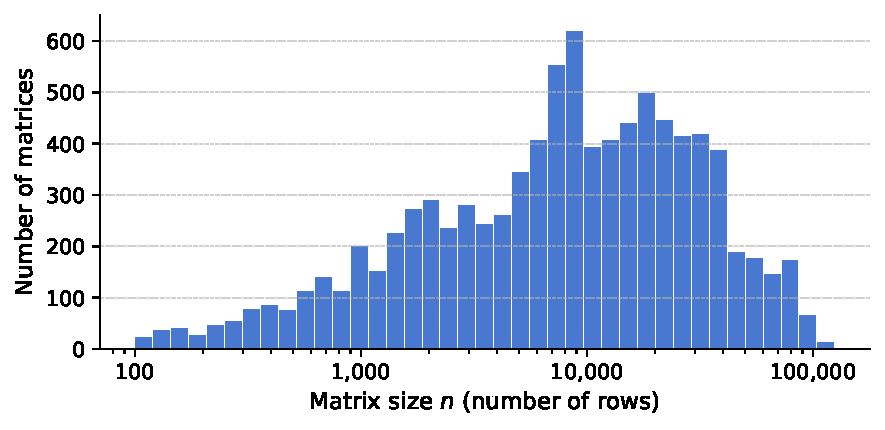
\includegraphics[width=0.85\textwidth]{figures/dataset_size_histogram.pdf}
  \caption{Distribution of matrix sizes (number of rows $n$) for the main thesis dataset
           (9{,}711 matrices, Campaigns~1--4). The $x$-axis uses a logarithmic scale.}
  \label{fig:dataset-sizes}
\end{figure}

\section{Feature Engineering}\label{sec:features}

The matrix features provided to the MLP branch complement the visual information captured by the CNN, and the choice of features can independently influence prediction quality.
The next section introduces the feature sets used in this thesis and how they differ from the MM-AutoSolver approach.

\subsection{MM-AutoSolver Reference Features}\label{subsec:features-mm}

The MM-AutoSolver paper~\cite{xiong2025mmautosolver} extracts 17 numerical features from each
matrix, listed in Table~\ref{tab:features-mm}.
These features are used in the re-implemented baseline (\texttt{mm\_baseline}) to allow a direct
comparison under the paper's original feature assumptions.

\begin{table}[H]
  \centering
  \caption{17 numerical features used in MM-AutoSolver~\cite{xiong2025mmautosolver}.}
  \label{tab:features-mm}
  \begin{tabular}{clp{7cm}}
    \toprule
    \# & Name & Description \\
    \midrule
    0  & \texttt{row\_num}                  & Number of rows $n$ \\
    1  & \texttt{nnz}                       & Total number of non-zeros \\
    2  & \texttt{nnz\_ratio}                & Fill ratio $\mathit{nnz}/n^2$ \\
    3  & \texttt{nnz\_lower}                & Non-zeros in strict lower triangle \\
    4  & \texttt{nnz\_upper}                & Non-zeros in strict upper triangle \\
    5  & \texttt{nnz\_diagonal}             & Number of non-zero diagonal entries \\
    6  & \texttt{ave\_nnz\_row}             & Average non-zeros per row ($\mathit{nnz}/n$) \\
    7  & \texttt{max\_nnz\_row}             & Maximum non-zeros in any single row \\
    8  & \texttt{arr\_nnz\_rows}            & Variance of per-row non-zero counts \\
    9  & \texttt{max\_value}                & Maximum absolute off-diagonal entry \\
    10 & \texttt{max\_value\_diagonal}      & Maximum absolute diagonal entry \\
    11 & \texttt{diagonal\_dominance\_ratio}& Fraction of rows where $|a_{ii}| > \sum_{j \neq i}|a_{ij}|$ \\
    12 & \texttt{is\_symmetry}              & 1 if $\|A - A^\top\|_F / \|A\|_F < 0.01$, else 0 \\
    13 & \texttt{pattern\_symmetry}         & Fraction of non-zero positions mirrored in $A^\top$ \\
    14 & \texttt{value\_symmetry}           & $1 - \|A - A^\top\|_F / \|A\|_F$ \\
    15 & \texttt{row\_variability}          & $\log(1 + \max_i(\max_j|a_{ij}| / \min_j|a_{ij}|))$ \\
    16 & \texttt{col\_variability}          & Same as above computed column-wise \\
    \bottomrule
  \end{tabular}
\end{table}

\subsection{Original 14 Features}\label{subsec:features-14}

The 14 features extracted from each matrix, shown in Table~\ref{tab:features-14}, are grouped by the matrix property they capture.
Features 0--2 describe size and sparsity (matrix dimension, non-zero count, and fill ratio).
Feature 3 captures symmetry via the asymmetry ratio.
Features 4 and 9 characterise diagonal dominance, which is relevant for the stability of ILU-based preconditioners~\cite{meijerink1977iterative, saad2003iterative}.
Features 5--8 encode magnitude and scaling information,
and features 10--13 capture structural properties such as bandwidth, diagonal fill, and row-norm variation.
While the covered property groups overlap with those in MM-AutoSolver,
the specific formulations differ in order to explore whether alternative encodings of the same matrix characteristics lead to better solver predictions.

\begin{table}[h]
  \centering
  \caption{Original 14 matrix features used in the single-channel experiments.}
  \label{tab:features-14}
  \begin{tabular}{cll}
    \toprule
    \textbf{\#} & \textbf{Name} & \textbf{Description} \\
    \midrule
    0  & $\log(1+n)$                     & Matrix size (number of rows) \\
    1  & $\log(1+\text{nnz})$            & Number of non-zero entries \\
    2  & $\text{nnz}/n^2$                & Density (fill ratio) \\
    3  & $\|A - A^\top\|_F / \|A\|_F$   & Asymmetry measure \\
    4  & $\text{mean}(|d_i| / \sum|r_i|)$ & Mean diagonal dominance \\
    5  & $\|A\|_F / n$                   & Frobenius norm per row \\
    6  & $\text{tr}(A) / n$              & Normalised trace \\
    7  & $\max|a_{ij}| / \text{mean}|a_{ij}|$ & Relative maximum entry \\
    8  & $\log(1 + \rho(A))$             & Log spectral radius \\
    9  & $\log(1 + \kappa_\text{diag})$  & Diagonal condition number proxy \\
    10 & $\text{bw} / n$                 & Normalised bandwidth \\
    11 & $\text{nnz}_\text{diag} / n$    & Fraction of non-zero diagonal entries \\
    12 & $\text{CV}(\|r_i\|)$            & Row norm coefficient of variation \\
    13 & $\|A - D\|_F / \|A\|_F$        & Off-diagonal Frobenius fraction \\
    \bottomrule
  \end{tabular}
\end{table}

\subsection{Extended 20-Feature Set}\label{subsec:features-20}

During experimentation, six additional features were introduced to address specific prediction weaknesses observed in Campaign~1,
expanding the feature vector to 20 entries (Table~\ref{tab:features-6}).
Features 14 and 15 improve the separation between CG-type and GMRES-type solvers by encoding the sign structure of off-diagonal
entries and the fraction of positive diagonal entries, both of which correlate with matrix definiteness~\cite{saad2003iterative}.
Feature 16 distinguishes structurally symmetric from truly asymmetric matrices, helping to separate \texttt{gmres+gamg} from \texttt{fgmres+gamg} predictions.
Features 17 and 19 target ILU preconditioner stability: the minimum per-row diagonal dominance detects the single worst-case
row for ILU breakdown, while the variance of dominance ratios captures patchy instability that the mean alone misses.
Feature 18 encodes whether the non-zero structure is grid-like or unstructured, which is a strong predictor of GAMG suitability~\cite{stuben2001review}.

\begin{table}[H]
  \centering
  \caption[Six additional matrix features introduced in Campaign~2.]{The 6 additional matrix features introduced in Campaign~2, expanding the feature vector from 14 to 20 entries.}
  \label{tab:features-6}
  \begin{tabular}{cll}
    \toprule
    \textbf{\#} & \textbf{Name} & \textbf{Description} \\
    \midrule
    14 & \texttt{neg\_offdiag\_frac}   & Fraction of off-diagonal entries that are negative \\
    15 & \texttt{pos\_diag\_frac}      & Fraction of strictly positive diagonal entries \\
    16 & \texttt{struct\_sym\_frac}    & Fraction of $(i,j)$ entries with a matching $(j,i)$ entry \\
    17 & \texttt{min\_diag\_dominance} & $\min_i |d_i| / \sum|a_{ij}|_{j \neq i}$ \\
    18 & \texttt{nnz\_per\_row\_cv}    & Coefficient of variation of per-row non-zero counts \\
    19 & \texttt{diag\_dom\_variance}  & Variance of per-row diagonal dominance ratios \\
    \bottomrule
  \end{tabular}
\end{table}

\section{Image Representations}\label{sec:image-modes}

Image representation is an interesting topic within the thesis approach of improving prediction accuracy,
as different downsampling methods store completely different data within the image later read by the CNN.
Thus, several different downsampling methods were implemented, as shown in Table~\ref{tab:image-modes}, including
the RCM (Reverse Cuthill--McKee) reordering~\cite{cuthill1969reducing} method which permutes matrix rows and columns to reduce bandwidth before rendering.
This reordering is applied solely for image generation and is not passed to the solver, as the original matrix is used unchanged during benchmarking.

\begin{table}[h]
  \centering
  \caption[The 14 image modes evaluated in the single-channel experiments.]{The 14 image modes evaluated in the single-channel experiments. The six \texttt{rcm\_*} variants apply Reverse Cuthill--McKee reordering to the matrix before rendering with the corresponding base mode.}
  \label{tab:image-modes}
  \begin{tabular}{lp{8.5cm}}
    \toprule
    \textbf{Mode} & \textbf{Description} \\
    \midrule
    \texttt{binary}           & 1 where any non-zero falls in a pixel cell, 0 elsewhere \\
    \texttt{density}          & Non-zero count per cell divided by cell area, normalised to $[0,1]$ \\
    \texttt{log\_density}     & $\log(1 + \text{count})$ per cell, normalised to $[0,1]$ \\
    \texttt{magnitude}        & Mean absolute entry value per cell, normalised to $[0,1]$ \\
    \texttt{sign}             & Mean sign per cell: positive $\to 1$, negative $\to 0$, mixed $\to 0.5$ \\
    \texttt{signed\_magnitude}& $\text{sign}(a) \cdot \log(1+|a|)$ per cell, normalised to $[0,1]$ with $0.5 = 0$ \\
    \texttt{symmetry}         & $|A - A^\top|$ per cell, normalised to $[0,1]$ \\
    \texttt{diagonal}         & Off-diagonal entries $= 0.5$, diagonal entries $= 1.0$ \\
    \midrule
    \texttt{rcm\_binary}           & \multirow{6}{*}{\parbox{8.5cm}{RCM-reordered variants of the above modes. Reverse Cuthill--McKee reordering reduces matrix bandwidth before rendering, grouping structurally related entries closer to the diagonal.}} \\
    \texttt{rcm\_density}          & \\
    \texttt{rcm\_log\_density}     & \\
    \texttt{rcm\_magnitude}        & \\
    \texttt{rcm\_sign}             & \\
    \texttt{rcm\_signed\_magnitude}& \\
    \bottomrule
  \end{tabular}
\end{table}

Throughout the thesis, experiments are referred to using the naming convention
\texttt{<mode>\_<size>} for single-channel and \texttt{<mode1>\_\_<mode2>\_<size>} for dual-channel experiments,
where \texttt{<size>} is the image resolution in pixels.
For example, \texttt{magnitude\_64} denotes magnitude downsampling at 64\,px,
and \texttt{magnitude\_\_rcm\_log\_density\_128} a dual-channel run with magnitude and
RCM log-density modes at 128\,px.

\section{Model Architecture}\label{sec:architecture}

The model consists of two sub-models combined into one prediction model.
The two branches are an MLP that processes previously defined matrix features, and a CNN that processes pre-rendered images.
Outputs are then concatenated and passed to a shared classification head, which produces the probability distribution over the 19 solver-preconditioner pairs.
Concatenation was chosen over element-wise addition as it is the more common fusion practice~\cite{baltruvsaitis2018multimodal} and gives the classification head greater freedom in weighting contributions from each branch independently.
Two different model sizes are introduced to evaluate the effect of model capacity.
The CNN branch supports a single image channel and a dual-channel variant that accepts two different images as input.

\subsection{CNN Branch}\label{subsec:cnn-branch}

The CNN branch accepts an image of the size $(C \times H \times W)$ as input,
where  $C = 1$ for single-channel and $C = 2$ for dual-channel experiments,
and $H = W \in \{64, 128\}$ depending on the image resolution.

The branch begins with an initial convolution block, a $3 \times 3$ convolution with
$c$ output channels, followed by batch normalisation~\cite{ioffe2015batch} and ReLU activation, and a
$2 \times 2$ max-pooling layer that halves the spatial dimensions.
This is then followed by two residual blocks (three for the large model variant),
where each one is separated by a $2 \times 2$ max-pooling step.
Each residual block consists of two $3 \times 3$ convolutions with batch normalisation
and a skip connection~\cite{he2016deep}: $\mathbf{y} = \text{ReLU}(\mathbf{x} + \text{block}(\mathbf{x}))$.

After the convolutional stack, an adaptive average pooling layer reduces the spatial
dimensions to a fixed $4 \times 4$ output regardless of input resolution.
The result is then flattened and passed through a fully connected layer to produce a
fixed-size CNN embedding of dimension $d_{\text{CNN}}$.

Two model sizes are defined:
\begin{itemize}
  \item \textbf{Small}: $c = 64$ channels, 2 residual blocks, $d_{\text{CNN}} = 256$,
        dropout $p = 0.3$, ${\approx}0.5$\,M parameters.
  \item \textbf{Large}: $c = 128$ channels, 3 residual blocks, $d_{\text{CNN}} = 512$,
        dropout $p = 0.4$, ${\approx}2$\,M parameters.
\end{itemize}

\subsection{MLP Branch}\label{subsec:mlp-branch}

The MLP branch processes the vector of scalar matrix features
$\mathbf{f} \in \mathbb{R}^{n_{\text{feat}}}$, where $n_{\text{feat}} \in \{14, 20\}$
depending on the experimental campaign.

It consists of two fully connected layers with ReLU activations:
\[
  \mathbf{h} = \text{ReLU}(W_2\,\text{ReLU}(W_1 \mathbf{f} + b_1) + b_2),
  \quad W_1, W_2 \in \mathbb{R}^{d_{\text{MLP}} \times \cdot}
\]
The hidden dimension is $d_{\text{MLP}} = 64$ (small model) or $d_{\text{MLP}} = 128$
(large model).
No dropout is applied in this branch, as the features are already low-dimensional and the risk of overfitting is low.

\subsection{Fusion and Classification Head}\label{subsec:fusion}

The outputs of the two branches are concatenated:
\[
  \mathbf{z} = [\mathbf{c}_{\text{CNN}};\, \mathbf{h}_{\text{MLP}}]
  \in \mathbb{R}^{d_{\text{CNN}} + d_{\text{MLP}}}
\]
and passed through a two-layer classification head with ReLU activation and dropout~\cite{srivastava2014dropout},
producing logits over the 19 solver-preconditioner classes:
\[
  \hat{\mathbf{y}} = W_{\text{out}}\,\text{ReLU}(W_{\text{head}}\,\mathbf{z} + b_{\text{head}}) + b_{\text{out}}
\]
The head hidden dimension is 128 (small) or 256 (large).

This concatenation-based fusion differs from the MM-AutoSolver~\cite{xiong2025mmautosolver} approach,
which uses an element-wise addition of the CNN and MLP outputs.
Concatenation is more flexible as the classification head here can learn arbitrary weighting
of the two branches, whereas element-wise addition requires both branches to produce
outputs with the same size and a compatible representation.

When \texttt{no\_cnn=True}, the CNN branch is disabled entirely and only the MLP branch
feeds into the head, serving as the \texttt{nocnn} feature-only baseline.

\section{Training Procedure}\label{sec:training}

All models are trained with the AdamW optimiser~\cite{loshchilov2019decoupled}
at a learning rate of $3 \times 10^{-4}$ and weight decay of $10^{-3}$.
A cosine annealing schedule~\cite{loshchilov2017sgdr} reduces the learning rate to zero over the full
training run of 256 epochs.
Batches of size 256, or in the dual-channel case 64 due to memory restrictions, are drawn
from the training split with shuffling.

The base loss is cross-entropy over the 19 classes.
In Campaigns~2 and~4 an additional convergence penalty is added:
\[
  \mathcal{L} = \mathcal{L}_{\text{CE}} + \lambda \sum_{k \notin \mathcal{C}(A)} \hat{p}_k
\]
where $\mathcal{C}(A)$ is the set of solvers that converged for matrix $A$,
$\hat{p}_k$ is the predicted probability for solver $k$, and $\lambda = 1.0$.
This directly penalises probability mass assigned to diverging solvers and is expected to reduce failure rates.

The dataset is split into 90\% training and 10\% validation data using a stratified split
with seed 42, ensuring each class is represented proportionally in both splits.
Checkpoints are saved every 5 epochs and the checkpoint from the final epoch is used for evaluation.